\section{Parts Reference}

In this section we list all the necessary parts for the assembly of the robot hand. The parts are divided in two categories: i) the robot finger parts and ii) the robot base parts. The second category contains the parts for the AX12 Dynamixel servo base, as well as a second base for a standard RC servo, like the Hitec HS-311. The parts that can be constructed using a 3D-printer, are presented in section 5.4.  As you can see below, the three tables contain the names of the Solidworks part files, as well as their quantity and usage. To facilitate the identification of each part, we also provide images of the models. 

\subsection{Robot Finger}

\begin{table}[h!]
\centering
\scalebox{0.9}{
	\begin{tabular}{ | l | l | l |}
	\hline
 	\multicolumn{3}{|c|}{\bf{Robot Finger}} \\
	\hline
	{\bf{Part Name}} & {\bf{Qty}} & {\bf{Description}}\\ \hline
	FingerBase1 & 8 &Acrylic Part for Finger Base   \\ \hline
    	FingerBase2 & 4 & Acrylic Part for Finger Base \\ \hline
    	FingerBase3 & 4 & Acrylic Part for Finger Base \\ \hline
    	FingerMCP & 4 & Acrylic Part for MCP \\ \hline
    	FingerPIP &  4 & Acrylic Part for PIP\\ \hline
    	FingerDIP &  4 & Acrylic Part for DIP \\ \hline
    	TubeplateMCP & 8 & Acrylic Part for Base of Tubes for MCP\\ \hline
    	Tubeplate & 12 &  Acrylic Part for Base of Tubes for Phalanges\\ \hline
    	tubeMCP & 8 & Cotton Swab Tube for MCP [d:2mm, D:2.5mm, L:8mm]  \\ \hline
    	tubePIP & 8 & Cotton Swab Tube for PIP [d:2mm, D:2.5mm, L:26mm]  \\ \hline
    	tubeDIP & 8 & Cotton Swab Tube for DIP [d:2mm, D:2.5mm, L:10mm]  \\ \hline
	Joint1 & 4 & Silicone Sheet, 60A Durometer  [(35x18x3)mm]\\ \hline
    	Joint2 & 4 & Silicone Sheet, 60A Durometer [(39x18x4)mm]\\ \hline
    	M3Washer &  20 & Fastener \\ \hline
	M3x12 &  8 &  Fastener  \\ \hline
    	M3Nut &  9 & Fastener \\ \hline
    	pulley & 4 & V-Groove Sealed Ball Bearing [d:3mm, D:12mm, B:4mm, Deepness:1.2mm] \\ \hline
	Dyneema Fishing Line & 1 & Tendon Routing [D:0.4mm, Strength:41.5kg] \\ \hline
	Rubber Foam Tape & 1 & [Width:10mm, Thickness:4mm] \\ \hline
	Anti-Slip Tape & 1 & 3M Gripping Material [Width:25mm] \\ \hline
	Self-Adhesive Tape & 1 & 3M Scotch 23 [Width:20mm] \\ \hline
    	\end{tabular}
}
\end{table}

\newpage

\begin{center}
\begin{tikzpicture}
\node [mybox] (box){%
	\begin{tabular}{ c c c c}
		
\includegraphics[width=2cm]{figures/Parts/Finger_Base_1.jpg} &
		
\includegraphics[width=1cm]{figures/Parts/FingerBase_2.jpg} &
		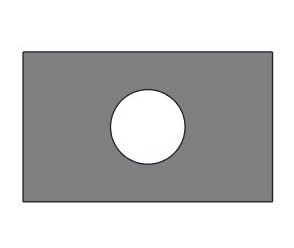
\includegraphics[width=1cm]{figures/Parts/FingerBase_3.jpg}	&
		
\includegraphics[width=1.5cm]{figures/Parts/FingerMCP.jpg} \\
		FingerBase1 &  FingerBase2 & FingerBase3 & FingerMCP \\ \\
		
\includegraphics[width=1.8cm]{figures/Parts/FingerPIP.jpg} &
		
\includegraphics[width=2.1cm]{figures/Parts/FingerDIP.jpg} &
		
\includegraphics[width=1.3cm]{figures/Parts/TubePlate_MCP.jpg} &
		
\includegraphics[width=2cm]{figures/Parts/TubePlate.jpg} \\
		FingerPIP & FingerDIP & TubeplateMCP & Tubeplate \\ \\
		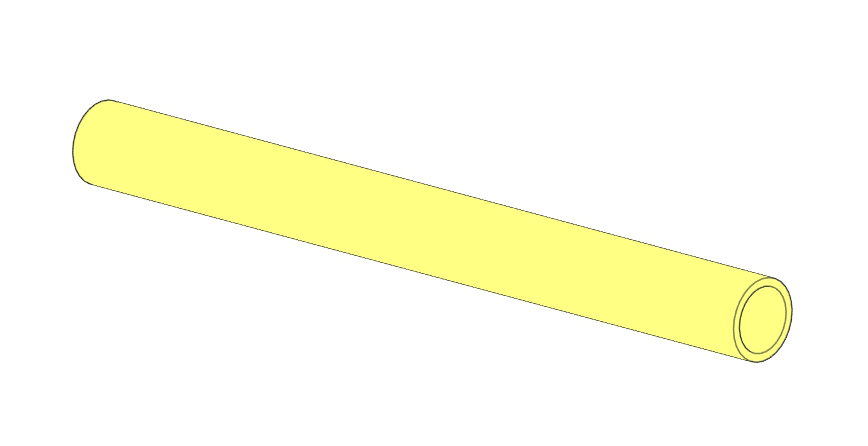
\includegraphics[width=2.5cm]{figures/Parts/Tube.png} &
		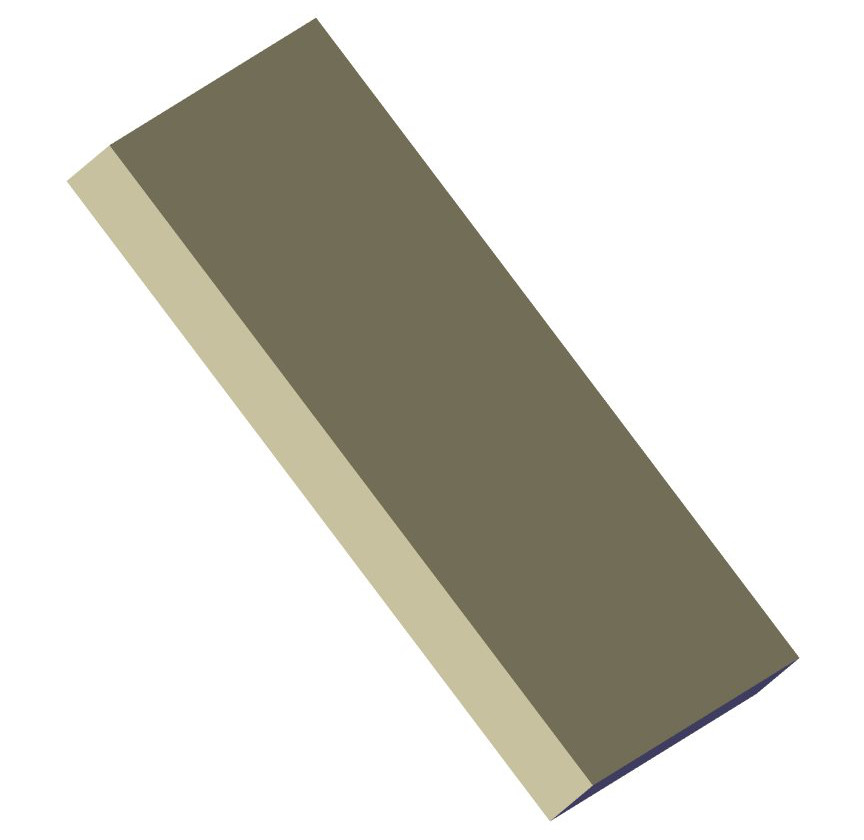
\includegraphics[width=2.5cm]{figures/Parts/SiliconeSheet.jpg} &
		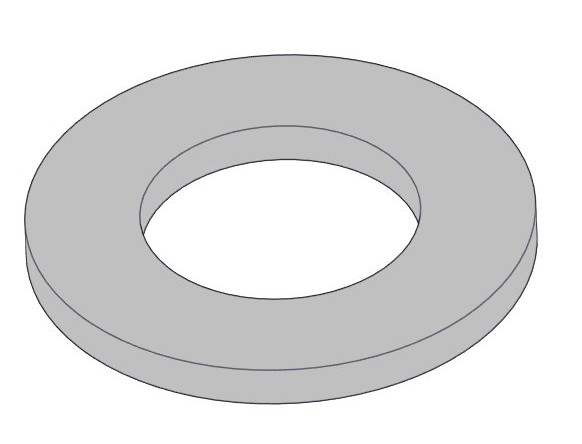
\includegraphics[width=0.9cm]{figures/Parts/WasherM3.jpg} &
		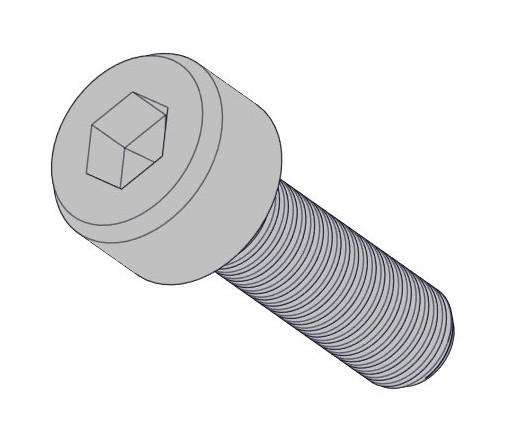
\includegraphics[width=1.8cm]{figures/Parts/ScrewM3x12.jpg} \\
		tubes &  Joint1, Joint2 & M3Washer & M3x12 \\ \\
		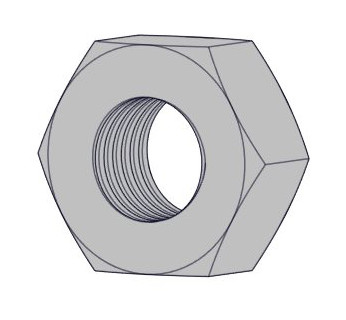
\includegraphics[width=1cm]{figures/Parts/NutM3.jpg} &
		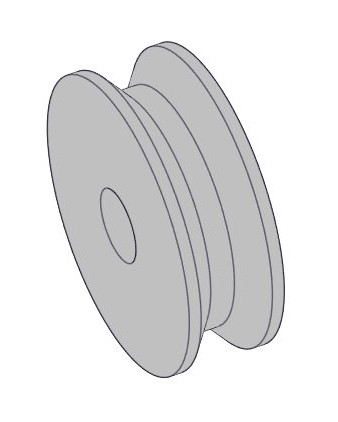
\includegraphics[width=1.4cm]{figures/Parts/Pulley.jpg} \\
		M3Nut & pulley  \\ \\
    	\end{tabular}
};
\node[mytitle, right=10pt] at (box.north west) {Parts};
\end{tikzpicture}%
\end{center}

\newpage

\subsection{Robot Hand Base for AX12 Servo}

\begin{table}[h!]
\centering
\scalebox{0.8}{
	\begin{tabular}{ | l | l | l |}
	\hline
 	\multicolumn{3}{|c|}{{\bf{Robot Hand Base for AX12 Servo}}} \\
	\hline
        {\bf{Part Name}} & {\bf{Qty}} & {\bf{Description}}\\ \hline
    	TopPlate & 2 & Acrylic Part of Robot Hand Base  \\ \hline
    	MiddlePlate & 1 & Acrylic Part of Robot Hand Base\\ \hline
    	DifferentialDisk & 2 & Acrylic Part of Differential Mechanism \\ \hline
    	BottomPlateAX12& 2 & Acrylic Part of Robot Hand Base \\ \hline
    	BearingBase & 4 & Acrylic Part of Robot Hand Base \\ \hline
    	AX12Base & 1 & Acrylic Part of Actuator Base \\ \hline
    	flangeAX12 \#1 & 1 & Acrylic Part of Flange \\ \hline
    	flangeAX12 \#2 & 1 & Acrylic Part of Flange \\ \hline
    	flangeAX12 \#3 & 1 & Acrylic Part of Flange \\ \hline
    	servoPulleyAX12 \#1 & 1 & Acrylic Part of Actuator Pulley \\ \hline    	
    	servoPulleyAX12 \#2 & 1 & Acrylic Part of Actuator Pulley \\ \hline
    	servoPulleyAX12 \#3 & 1 & Acrylic Part of Actuator Pulley \\ \hline
    	PCBMount & 1 & Acrylic Part for PCB \\ \hline    	    	    	    	
	Dyneema Fishing Line & 1 & Tendon Routing [D:0.4mm, Strength:41.5kg] \\ \hline
	Rubber Foam Tape & 1 & Tape for Fingertips [Width:10mm, Thickness:4mm] \\ \hline
	Anti-Slip Tape & 1 & 3M Gripping Material [Width:25mm] \\ \hline
    	AX12 & 1 & Robotis Actuator Dynamixel AX-12A  \\ \hline
    	pulley & 1 & V-Groove Sealed Ball Bearing [d:3mm, D:12mm, B:4mm, Deepness:1.2mm] \\ \hline
    	PlasticSpacer & 2 & Fastener [d:3.1mm, D:6mm, L:2mm] \\ \hline
    	M3Spacer30 & 8 & Fastener, Spacer M3 [L:30mm] \\ \hline
    	M3Spacer25 & 4 & Fastener, Spacer M3 [L:25mm] \\ \hline
    	M3Spacer10 & 4 & Fastener, Spacer M3  [L:10mm] \\ \hline
	M3ThreadedRod & 4 & Fastener, M3 Threaded Rod [L:20mm] \\ \hline	
    	M3x10 & 16 & Fastener, M3 [L:10mm] \\ \hline
    	M3x20 & 1 & Fastener, M3 [L:20mm] \\ \hline
    	M3Washer &  13 & Fastener, M3 [D:7.5, L:0.5mm] \\ \hline
    	M3Nut &  1 & Fastener, M3 Hex Nut \\ \hline
    	M2x8 & 8 & Fastener, M2 [L:8mm] \\ \hline
    	M2x6 & 2 & Fastener, M2 [L:6mm] \\ \hline
    	M2Nut & 8 & Fastener, M2 Hex Nut \\ \hline
	M2.5x15 & 1 & Fastener, M2.5 for AX12 [L:15mm] \\ \hline
    	\end{tabular}
}
\end{table}

\vspace{0.2cm}

\begin{center}
\begin{tikzpicture}
\node [mybox] (box){%
	\begin{tabular}{ c c c c}
		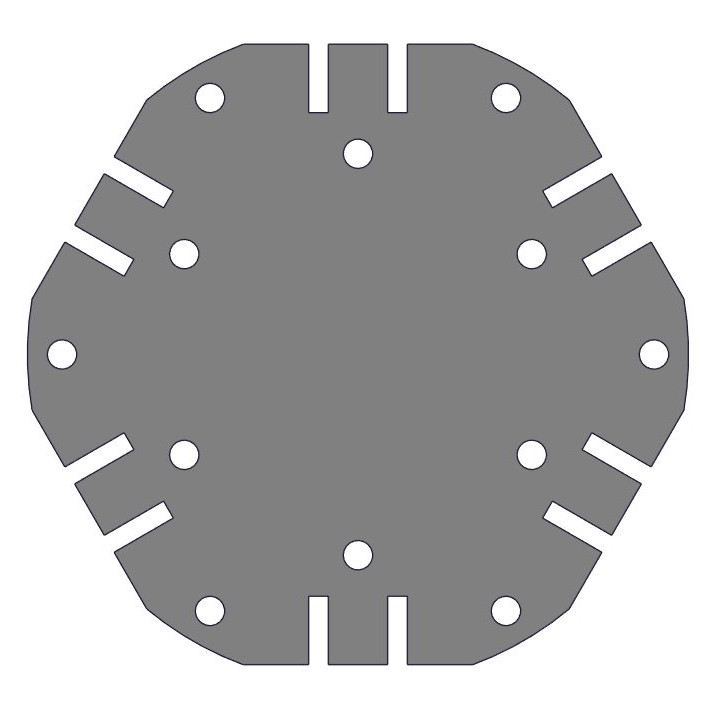
\includegraphics[width=4cm]{figures/Parts/TopPlate.jpg} &
		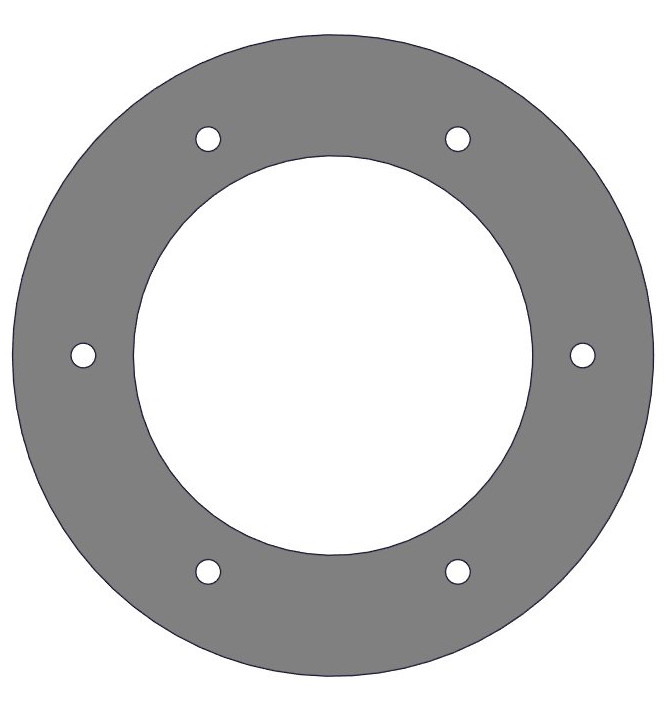
\includegraphics[width=4cm]{figures/Parts/MiddlePlate_1.jpg} &
		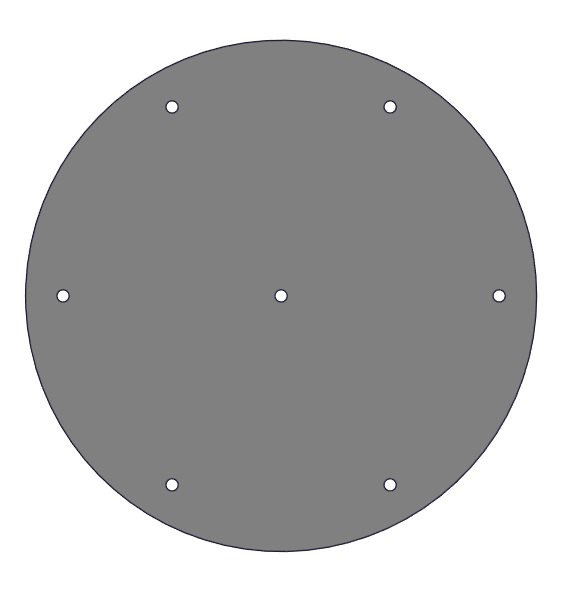
\includegraphics[width=2.8cm]{figures/Parts/DifferentialDisk.jpg} \\ 
		TopPlate & MiddlePlate &   DifferentialDisk \\
		
\includegraphics[width=4cm]{figures/Parts/BottomPlate.png} &
		
\includegraphics[width=1.6cm]{figures/Parts/BearingBase.jpg} &
		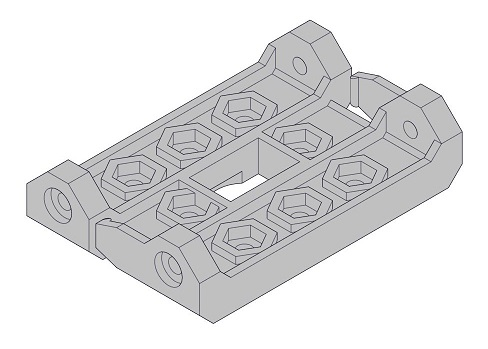
\includegraphics[width=3.2cm]{figures/Parts/DynamixelBase.jpg} \\
		BottomPlateAX12 & BearingBase &  AX12Base \\
    	\end{tabular}
};
\node[mytitle, right=10pt] at (box.north west) {Parts};
\end{tikzpicture}%
\end{center}

\newpage

\begin{center}
\begin{tikzpicture}
\node [mybox] (box){%
	\begin{tabular}{ c c c }
		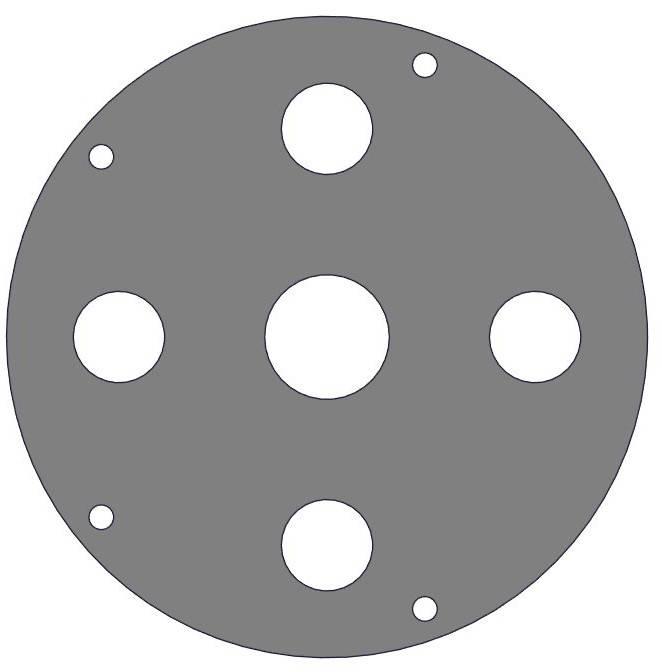
\includegraphics[width=4.2cm]{figures/Parts/Flange1.jpg} &
		
\includegraphics[width=4cm]{figures/Parts/Flange2.jpg} & 
		
\includegraphics[width=4cm]{figures/Parts/Flange3.jpg} \\
		flangeAX12 \#1 & flangeAX12 \#2 &  flangeAX12 \#3\\ \\
		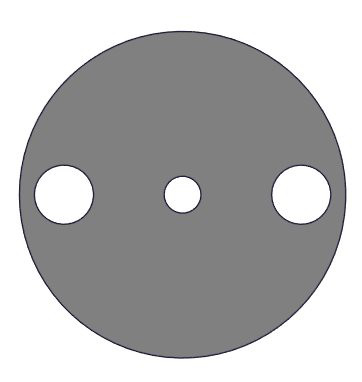
\includegraphics[width=2cm]{figures/Parts/servoPulley1.jpg} &
		
\includegraphics[width=1cm]{figures/Parts/servoPulley2.jpg} &
		
\includegraphics[width=2.1cm]{figures/Parts/servoPulley3.jpg} \\
		servoPulleyAX12 \#1 & servoPulleyAX12 \#2 & servoPulleyAX12 \#3 \\ \\
		
\includegraphics[width=3cm]{figures/Parts/PCBMount.png} &		
		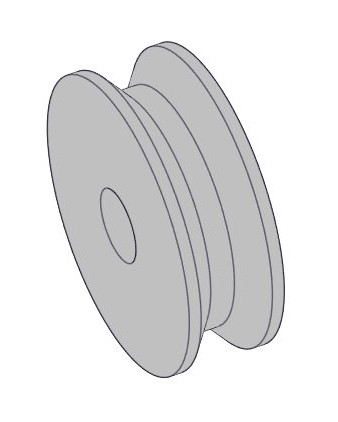
\includegraphics[width=1.4cm]{figures/Parts/Pulley.jpg} &
		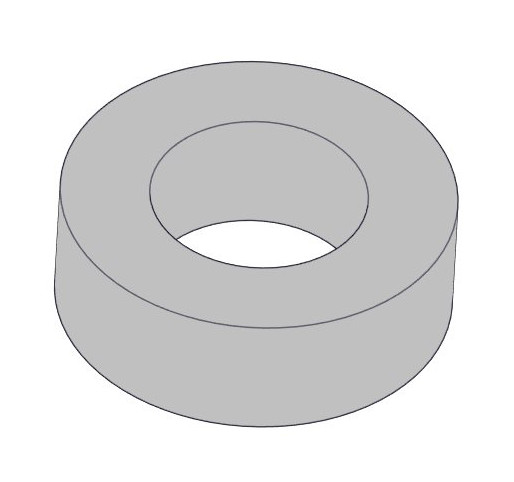
\includegraphics[width=1.2cm]{figures/Parts/PlasticSpacer.jpg} \\
 		PCBMount & pulley & PlasticSpacer \\ \\
		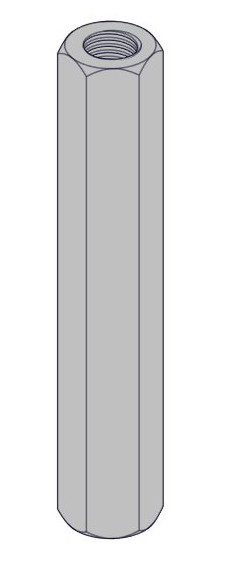
\includegraphics[width=1.4cm]{figures/Parts/M3Spacer30.jpg} &
		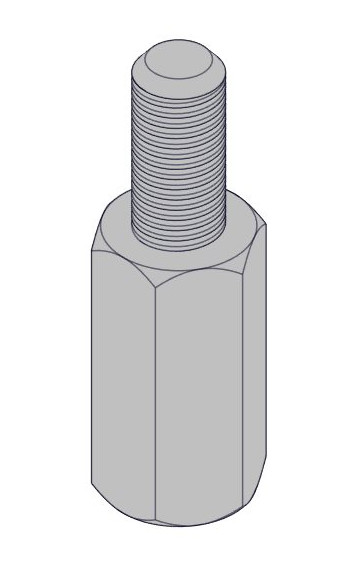
\includegraphics[width=1.4cm]{figures/Parts/M3Spacer10.jpg} &
		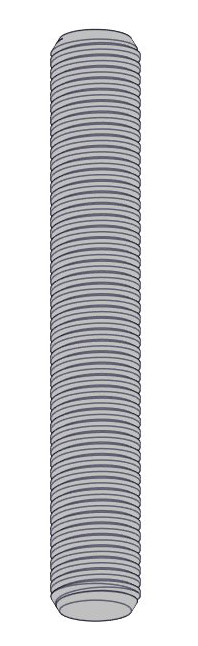
\includegraphics[width=1cm]{figures/Parts/M3ThreadRod.jpg} \\
		M3Spacer30, M3Spacer25 & M3Spacer10 &  M3ThreadedRod \\ \\
		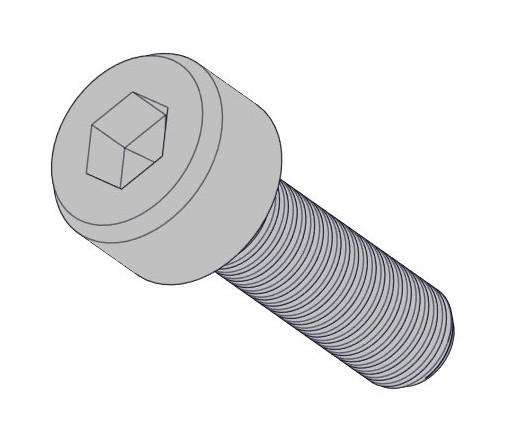
\includegraphics[width=1.8cm]{figures/Parts/ScrewM3x12.jpg} &
		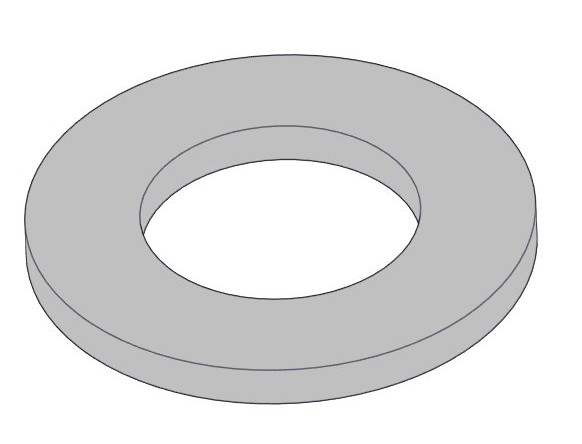
\includegraphics[width=0.9cm]{figures/Parts/WasherM3.jpg} &
		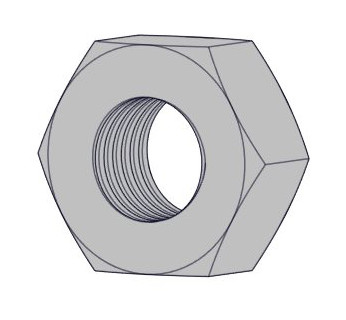
\includegraphics[width=1cm]{figures/Parts/NutM3.jpg} \\
		M3x10, M3x20 & M3Washer & M3Nut \\ \\
		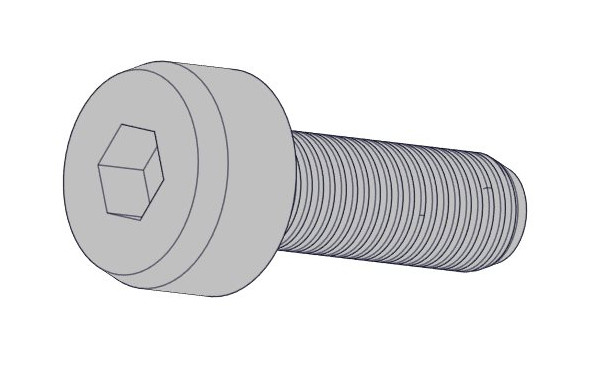
\includegraphics[width=1.6cm]{figures/Parts/M2x6.jpg} &		
		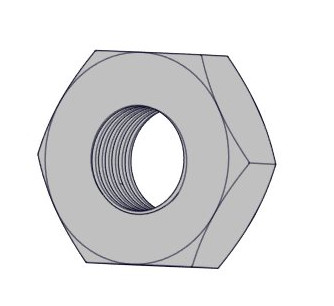
\includegraphics[width=1cm]{figures/Parts/M2Nut.jpg} \\
		M2x6, M2x8 & M2Nut\\ \\
    	\end{tabular}
};
\end{tikzpicture}%
\end{center}

\newpage

\subsection{Robot Hand Base for Standard Servo}

\begin{table}[h!]
\centering
\scalebox{0.8}{
	\begin{tabular}{ | l | l | l |}
	\hline
 	\multicolumn{3}{|c|}{{\bf{Robot Hand Base for Standard Servo}}} \\
	\hline
	{\bf{Part Name}} & {\bf{Qty}} & {\bf{Description}}\\ \hline
    	TopPlate & 2 & Acrylic Part of Robot Hand Base  \\ \hline
    	MiddlePlate & 1 & Acrylic Part of Robot Hand Base\\ \hline
    	DifferentialDisk & 2 & Acrylic Part of  Differential Mechanism \\ \hline
    	BottomPlateStdServo & 2 & Acrylic Part of Robot Hand Base \\ \hline
    	BearingBase & 4 & Acrylic Part of Robot Hand Base \\ \hline
    	stdServoBase & 6 & Acrylic Part of Actuator Base \\ \hline
    	flangeStdServo \#1 & 1 & Acrylic Part of Flange \\ \hline
    	flangeStdServo \#2 & 1 & Acrylic Part of Flange \\ \hline
    	flangeStdServo \#3 & 1 & Acrylic Part of Flange \\ \hline
    	servoPulleyStd \#1 & 1 & Acrylic Part of Actuator Pulley \\ \hline    	
    	servoPulleyStd \#2 & 1 & Acrylic Part of Actuator Pulley \\ \hline
    	servoPulleyStd \#3 & 1 & Acrylic Part of Actuator Pulley \\ \hline
    	PCBMount & 1 & Acrylic Part for PCB \\ \hline    	    	    	    	
	Dyneema & 1 & Tendon Routing [D:0.4mm, Strength:41.5kg] \\ \hline
	Rubber Foam Tape & 1 & [Width:10mm, Thickness:4mm] \\ \hline
	Anti-Slip Tape & 1 & 3M Gripping Material [Width:25mm] \\ \hline
    	Hitec HS-311 & 1 &  Actuator\\ \hline
    	pulley & 1 & V-Groove Sealed Ball Bearing [d:3mm, D:12mm, B:4mm, Deepness:1.2mm] \\ \hline
    	PlasticSpacer & 2 & Fastener [d:3.1mm, D:6mm, L:2mm] \\ \hline
    	M3Spacer30 & 8 & Fastener, Spacer M3 [L:30mm] \\ \hline
    	M3Spacer25 & 4 & Fastener, Spacer M3 [L:25mm] \\ \hline
    	M3Spacer10 & 4 & Fastener, Spacer M3 [L:10mm] \\ \hline
	M3ThreadedRod & 4 & Fastener, M3 Threaded Rod [L:20mm]  \\ \hline	
    	M3x10 & 16 & Fastener, M3 [L:10mm] \\ \hline
    	M3x12 & 6 & Fastener, M3 [L:10mm] \\ \hline
    	M3x20 & 1 & Fastener, M3 [L:20mm] \\ \hline
    	M3Nut &  7 & Fastener, M3 Hex Nut \\ \hline
    	M3Washer &  18 & Fastener, M3 [D:7.5mm, L:0.5mm] \\ \hline
    	\end{tabular}
}
\end{table}

\vspace{0.2cm}

\begin{center}
\begin{tikzpicture}
\node [mybox] (box){%
	\begin{tabular}{ c c c }
		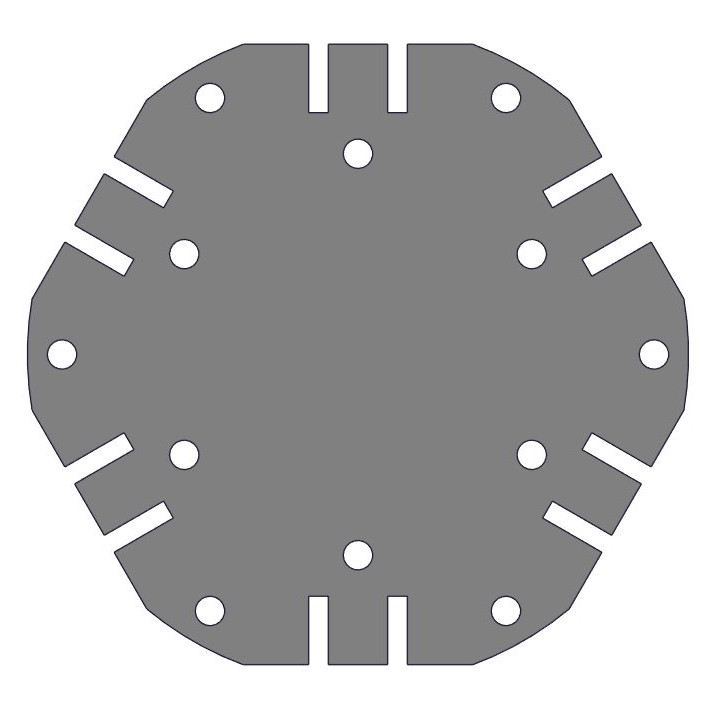
\includegraphics[width=4cm]{figures/Parts/TopPlate.jpg} &
		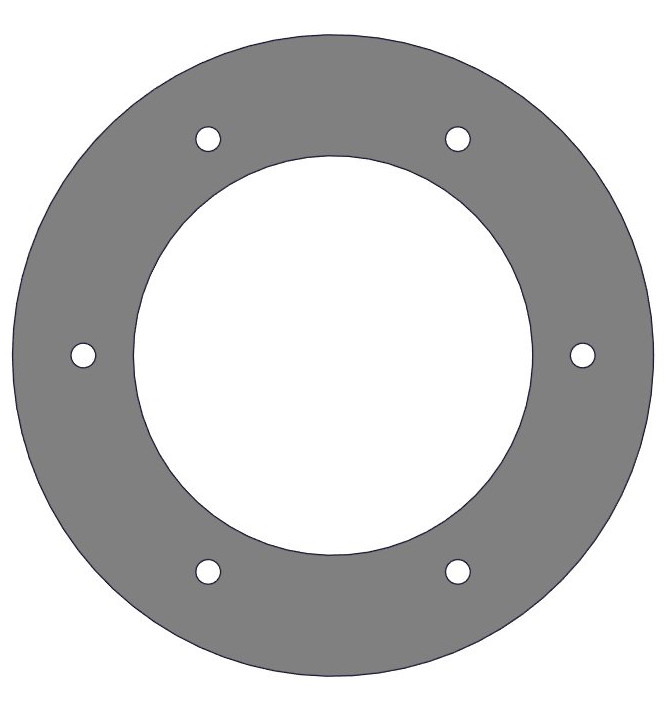
\includegraphics[width=4cm]{figures/Parts/MiddlePlate_1.jpg} & 
		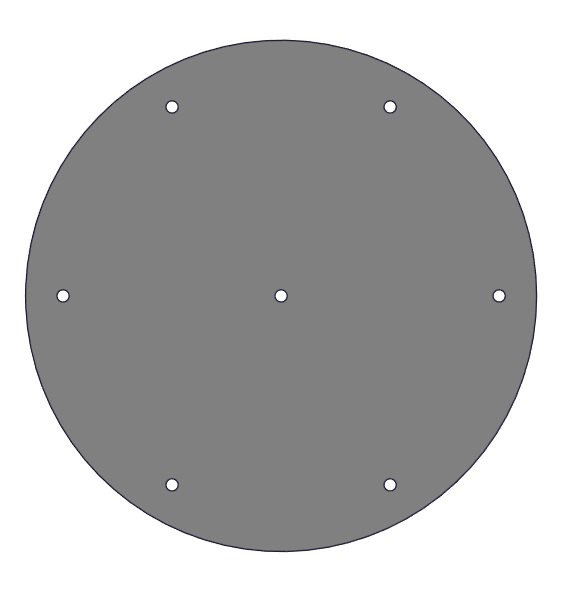
\includegraphics[width=2.8cm]{figures/Parts/DifferentialDisk.jpg} \\
		TopPlate & MiddlePlate & DifferentialDisk \\ \\
		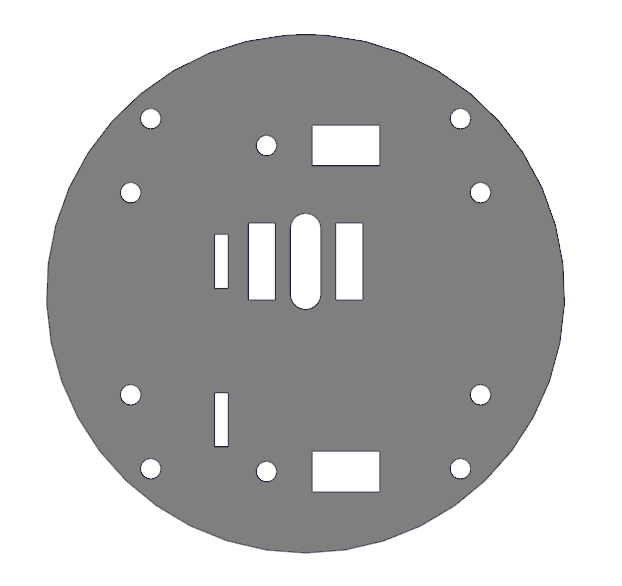
\includegraphics[width=4.4cm]{figures/Parts/BottomPlateStdServo.png} &
		
\includegraphics[width=1.6cm]{figures/Parts/BearingBase.jpg} &
		
\includegraphics[width=1.8cm]{figures/Parts/stdServoBase.jpg} \\
		BottomPlate & BearingBase & stdServoBase \\
    	\end{tabular}
};
\node[mytitle, right=10pt] at (box.north west) {Parts};
\end{tikzpicture}%
\end{center}

\newpage

\begin{center}
\begin{tikzpicture}
\node [mybox] (box){%
	\begin{tabular}{ c c c }
		
\includegraphics[width=4cm]{figures/Parts/flangeStdServo_part1.png} &
		
\includegraphics[width=4cm]{figures/Parts/flangeStdServo_part2.jpg} & 
		
\includegraphics[width=4.2cm]{figures/Parts/flangeStdServo_part3.png} \\
		flangeStdServo \#1 & flangeStdServo \#2 &  flangeStdServo \#3\\ \\
		
\includegraphics[width=2cm]{figures/Parts/servoPulleyStd1.jpg} &
		
\includegraphics[width=1.4cm]{figures/Parts/servoPulleyStd2.jpg} &
		
\includegraphics[width=2.1cm]{figures/Parts/servoPulleyStd3.jpg} \\
		servoPulleyStd \#1 & servoPulleyStd \#2 & servoPulleyStd \#3\\ \\
		
\includegraphics[width=3cm]{figures/Parts/PCBMount.png} &		
		\includegraphics[width=1.4cm]{figures/Parts/Pulley.jpg} &
		\includegraphics[width=1.2cm]{figures/Parts/PlasticSpacer.jpg} \\
		PCBMount & pulley & PlasticSpacer \\ \\
		\includegraphics[width=1.4cm]{figures/Parts/M3Spacer30.jpg} &
		\includegraphics[width=1.4cm]{figures/Parts/M3Spacer10.jpg} &
		\includegraphics[width=1cm]{figures/Parts/M3ThreadRod.jpg} \\
		 M3Spacer25, M3Spacer30 & M3Spacer10 & M3ThreadedRod \\ \\
		\includegraphics[width=1.8cm]{figures/Parts/ScrewM3x12.jpg} &
		\includegraphics[width=1cm]{figures/Parts/NutM3.jpg} &
		\includegraphics[width=0.9cm]{figures/Parts/WasherM3.jpg} \\
		M3x10, M3x12, M3x20 & M3Nut &  M3Washer\\ \\
    	\end{tabular}
};
\end{tikzpicture}%
\end{center}

\newpage

\subsection{3D Printer Parts}

The proposed robot hands can also be created with other materials like ABS, using 3D printing. The STL files in the CAD directory, are 
appropriate to be used with a 3D printer. The following table contains the required parts, as well as the names of the standard parts that they replace. 

\vspace{0.2cm}

\begin{table}[h!]
\centering
\scalebox{0.8}{
	\begin{tabular}{ | l | l |}
	\hline
 	\multicolumn{2}{|c|}{{\bf{3D Printer Parts}}} \\
	\hline
	{\bf{Part Name}} & {\bf{Replacing Parts}}\\ \hline
	FingerBase & FingerBase1, FingerBase2, FingerBase3, FingerMCP, TubePlateMCP parts  \\ \hline
    	FingerPIP & FingerPIP, TubePlate parts\\ \hline
    	FingerDIP & FingerDIP, TubePlate parts\\ \hline
    	TopPlate & TopPlate parts  \\ \hline
    	MiddlePlate & MiddlePlate part\\ \hline
    	DifferentialDisk & DifferentialDisk parts  \\ \hline
    	BottomPlateStdServo & BottomPlateStdServo, BearingBase parts \\ \hline
    	stdServoBase &  stdServoBase parts\\ \hline
	FlangeStdServo & flangeStdServo \#1, flangeStdServo \#2, flangeStdServo \#3 parts \\ \hline
    	BottomPlateAX12 & BottomPlateAX12,  BearingBase parts \\ \hline
    	FlangeAX12 & flangeAX12 \#1, flangeAX12 \#2, flangeAX12 \#3 parts \\ \hline
    	servoPulleyStd \#1-2 & servoPulleyStd \#1, servoPulleyStd \#2 parts\\ \hline    	
    	servoPulleyStd \#3 & servoPulleyStd \#3 part \\ \hline
    	servoPulleyAX12 \#1-2 & servoPulleyAX12 \#1, servoPulleyAX12 \#2 parts  \\ \hline    	
    	servoPulleyAX12 \#3 & servoPulleyAX12 \#3 parts  \\ \hline
    	PCBMount & PCBMount part  \\ \hline
    	\end{tabular}
}
\end{table}

\vspace{0.2cm}

\begin{center}
\begin{tikzpicture}
\node [mybox] (box){%
	\begin{tabular}{ c c c }
		\includegraphics[width=2cm]{figures/Parts/FingerBase.jpg} &
		\includegraphics[width=2.5cm]{figures/Parts/FingerPIP-3d.jpg} & 
		\includegraphics[width=2.5cm]{figures/Parts/FingerDIP-3d.jpg} \\
		FingerBase & FingerPIP & FingerDIP \\ \\
		\includegraphics[width=4.5cm]{figures/Parts/TopPlate-3d.jpg} &
		\includegraphics[width=4.5cm]{figures/Parts/MiddlePlate-3d.jpg} &
		\includegraphics[width=3cm]{figures/Parts/DifferentialDisk-3d.jpg} \\
		TopPlate & MiddlePlate & DifferentialDisk \\ \\
		\includegraphics[width=4.5cm]{figures/Parts/BottomPlateStdServoWithBearingBase.png} &
		\includegraphics[width=2.5cm]{figures/Parts/stdServoBase-3d.jpg} &
		\includegraphics[width=4.5cm]{figures/Parts/FlangeStdServo-3d.jpg} \\
		BottomPlateStdServo & stdServoBase & FlangeStdServo\\
    	\end{tabular}
};
\node[mytitle, right=10pt] at (box.north west) {3D Printer Parts};
\end{tikzpicture}%
\end{center}

\newpage

\begin{center}
\begin{tikzpicture}
\node [mybox] (box){%
	\begin{tabular}{ c c c }
		\includegraphics[width=4.5cm]{figures/Parts/BottomPlateAX12withBearingBase.png} &
		\includegraphics[width=4.5cm]{figures/Parts/FlangeAX12-3d.jpg} &
		\includegraphics[width=2cm]{figures/Parts/servoPulleyStd1-2-3d.jpg} \\
		BottomPlateAX12 & FlangeAX12 & servoPulleyStd \#1-2 \\ \\
		\includegraphics[width=2cm]{figures/Parts/servoPulleyStd3-3d.jpg} &
		\includegraphics[width=2cm]{figures/Parts/servoPulleyAX12_1-2.jpg} &
		\includegraphics[width=2cm]{figures/Parts/servoPulleyAX12_3.jpg} \\
		servoPulleyStd \#3  & servoPulleyAX12 \#1-2  & servoPulleyAX12 \#3 \\
		\includegraphics[width=2.5cm]{figures/Parts/PCBMount.png} & & \\
		PCBMount & &\\
    	\end{tabular}
};
\end{tikzpicture}%
\end{center}

\vspace{1cm}

In order to print the required parts we use the \href{https://download.lulzbot.com/AO-100/documentation/LulzBot-AO-100-brochure.pdf}{LulzBot AO-100 Desktop 3D Printer}. The Slic3r (a G-code generator) printer settings are shown in the following table. The settings are also containted in a file named RobotHand.ini. 

\vspace{1cm}

\begin{table}[h!]
\centering
\scalebox{1}{
	\begin{tabular}{ | l | l |}
	\hline
 	\multicolumn{2}{|c|}{{\bf{3D Printer Settings}}} \\ \hline
	{\bf{Parameter}} & {\bf{Value}} \\ \hline
	Layer Height & 0.4022 \\ \hline   
	First Layer Height & 100\% \\ \hline   
	Solid Layers, Top & 3 \\ \hline
	Solid Layers, Bottom & 3 \\ \hline
	Infill, Fill Density & 40\% \\ \hline
	Infill, Fill Pattern & Honeycomb \\ \hline
	Infill, Top/Bottom Fill Pattern & Rectilinear \\ \hline
	Brim, Brim Width & 2 mm \\ \hline
	Support Material, Pattern & Pillars \\ \hline
	Support Material, Pattern Spacing & 2.5mm \\ \hline
	Support Material, Pattern Angle & 0 deg \\ \hline
	Support Material, Interface Layers & 3 layers \\ \hline
	Support Material, Interface Pattern Spacing & 0mm \\ \hline
    	\end{tabular}
}
\end{table}

\newpage

\subsection{Before Building}

Before starting the construction of the robot hand you must prepare the parts and pay attention to the steps provided below: \\  \\
$\bullet$ Smooth the acrylic parts with sandpaper. \\ \\
$\bullet$ Treat the ABS parts with acetone (more information: \href{http://blog.reprap.org/2013/02/vapor-treating-abs-rp-parts.html}{RepRap: Blog}).\\ \\
$\bullet$ Cut the cotton swabs, to the appropriate size (following the parts reference dimensions). \\ \\
$\bullet$ Cut the silicone sheets, to the appropriate size (following the parts reference dimensions). \\ \\
$\bullet$ Group the parts according to the parts reference. \\ \\
$\bullet$ Pay always attention to the details having the following icon \Circled{!}.\\ \\
$\bullet$ Please note that the provided models do not have the actual size of the parts.\\ \\

\begin{center}
\begin{tikzpicture}
\node [mybox] (box){%
        \begin{tabular}{ c }
	\includegraphics[width=8cm]{figures/Parts/SilliconeCut.jpg} \\
        Cutting the silicone sheets with a cutter and a ruler.
	\end{tabular}
};
\end{tikzpicture}%
\end{center}